\documentclass[t,14pt]{beamer}
\setbeamersize{text margin left=8mm,text margin right=8mm}

\usepackage{xeCJK}
\setCJKmainfont{Noto Sans CJK SC}
\setCJKmonofont{Noto Sans Mono CJK SC}
\setCJKsansfont{Noto Sans CJK SC}
\CJKsetecglue{}

\usetheme[sectionpage=none,block=fill]{metropolis}
\usepackage{appendixnumberbeamer}

\usepackage{booktabs}
\usepackage[scale=2]{ccicons}

\usepackage{graphicx}
\usepackage{subcaption}
\captionsetup[subfigure]{subrefformat=simple,labelformat=simple}
\renewcommand\thesubfigure{(\alph{subfigure})}
\usepackage{caption}
\captionsetup[table]{skip=0mm}
\usepackage{float}
\usepackage{adjustbox}

\usepackage{enumerate}
\setlength{\leftmargini}{5pt}
\setlength{\leftmarginii}{8pt}
\setbeamertemplate{itemize item}[square]
\setbeamertemplate{itemize subitem}[circle]
\setbeamertemplate{itemize subsubitem}[triangle]

\usepackage[backend=biber,citestyle=numeric-comp,sorting=none]{biblatex}
\addbibresource{main.bib}
\renewcommand*{\bibfont}{\scriptsize}

\usepackage{amsmath}
\usepackage{amsfonts}
\usepackage{amssymb}
\usepackage{bm}

\usepackage{array}
\usepackage{tabularx}
\usepackage{multirow}
\usepackage{calc}


\newenvironment{lead}{
  \vspace*{8pt}
  \begin{beamercolorbox}[wd=\dimexpr\linewidth+20pt\relax,sep=8pt,shadow=false,rounded=false]{block body example}
}{
  \end{beamercolorbox}
}


\title{Deriving Machine Attention from Human Rationales}
%\subtitle{beamerテンプレート}
\author{@koreyou}
\date[]{2018/12/9}
\institute{EMNLP2018読み会@サイバーエージェント, 東京}
%\titlegraphic{\includegraphics[scale=0.3]{logo.png}}

% subject and keywords are embedded as PDF meta info
%\subject{}
\keywords{論文読み,自然言語処理,深層学習,機械学習}

\begin{document}

\frame{\titlepage}

\begin{frame}{Who am I?}
  \begin{columns}[onlytextwidth]
  \begin{column}{0.68\linewidth}
    \begin{itemize}
      \item 是枝祐太
      \item 某電機会社リサーチャー
      \item 研究歴
      \begin{itemize}
        \item 〜2015: 医療+ロボット(大学)
        \item 〜2016: ロボット+応用機械学習
        \item 〜現在: \alert{応用機械学習+自然言語処理}
      \end{itemize}
    \end{itemize}
  \end{column}
  \begin{column}{0.3\linewidth}
    \begin{itemize}
      \item[] \raisebox{-0.3\height}{
\includegraphics[width=6mm]{fig/GitHub-Mark-64px.png}} koreyou
      \item[] \raisebox{-0.3\height}{
\includegraphics[width=6mm]{fig/Twitter_Social_Icon_Square_Color.png}} koreyou\_
    \end{itemize}
    \vspace*{10mm}
    \only<1>{\adjincludegraphics[width=0.95\linewidth,valign=t]{fig/my_weight_1.png}}
    \only<2>{\adjincludegraphics[width=0.95\linewidth,valign=t]{fig/my_weight_2.png}}
  \end{column}
  \end{columns}
\end{frame}

\begin{frame}{tl;dr}
\begin{itemize}
\item Bat et al. 2018. Deriving Machine Attention from Human Rationales. EMNLP.
\item 目的:分類の根拠となった箇所のデータを用い低リソースドメインで分類精度向上
\item 手法:ドメイン非依存なRationale$\Rightarrow$attentionの変換を学習
\begin{itemize}
\item Rationale:人間が作成した分類の根拠となる記載箇所
\end{itemize}
\item 結果:観点付き評判分析の観点、ドメイン転移でベースラインを上回った
\end{itemize}
\end{frame}

\begin{frame}{Table of contents}
  \setbeamertemplate{section in toc}[sections numbered]
  \tableofcontents[hideallsubsections]
\end{frame}

\begin{frame}[c]
  \begin{center}
    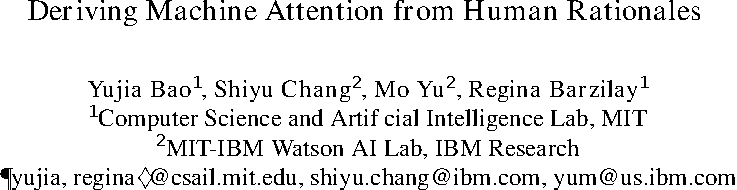
\includegraphics[width=\linewidth]{fig/title.pdf}    
  \end{center}
\end{frame}

\section{背景}
\frame[standout]{\insertsection}

\begin{frame}
\frametitle<1>{観点付き評判分析}
\frametitle<2>{Rationale (根拠、解釈)}

\begin{lead}
    \only<1>{観点付き評判分析をビークルに研究}
    \only<2>{根拠 (Rationale) 提示型AIが注目されている}
\end{lead}

\begin{overlayarea}{\linewidth}{120pt}
  \only<1>{
    \begin{itemize}
    \item 本研究は自然言語タスク全般に利用可能
    \begin{itemize}
        \item わかりやすさのために具体的なタスクを先に紹介
    \end{itemize}
    \item 観点付き評判分析 (Aspect-based sentiment analysis; ABSA)
    \begin{itemize}
        \item 入力文が各観点について肯定的か否定的かを分類
    \end{itemize}
    \item 本発表では``ドメイン''を``観点''と読みかえて理解
    \end{itemize}
  }
  \only<2>{
    \begin{itemize}
    \item Rationale$=$分類の\alert{根拠}となる記載箇所
    \begin{itemize}
        \item なぜその予測をしたかの\alert{解釈}を与えAIを\alert{説明可能}にする
    \end{itemize}
    \item Rationaleを提示する研究が注目されている\cite{lei_2016,ling_2017}
    \end{itemize}
  }
\end{overlayarea}
\begin{figure}[H]
    \centering
    \begin{overprint}
    \onslide<1>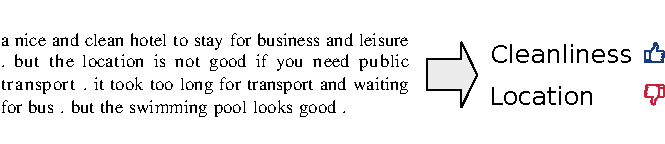
\includegraphics{fig/absa.pdf}%
    \onslide<2>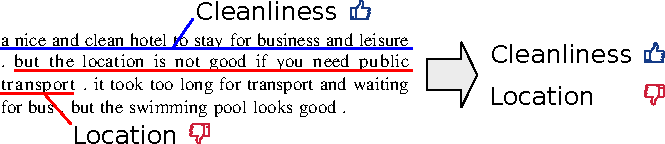
\includegraphics{fig/rationale.pdf}%
    \end{overprint}
\end{figure}
\end{frame}

\begin{frame}{研究目的}
\begin{lead}
    根拠データを使い低リソースドメインで精度向上
\end{lead}
\begin{itemize}
\item 分類の教師データに加え、なぜそのような分類をすべきかという\alert{根拠を学習に加える}ことで、\alert{少量のデータで高い分類精度}を実現できないか?
\end{itemize}
\end{frame}

\section{提案手法}
\frame[standout]{\insertsection}

\begin{frame}{文分類におけるAttention機構の活用}
\begin{lead}
    Attention機構により文分類の精度向上が図れる
\end{lead}
\begin{itemize}
\item プーリングとしてのattention機構
\begin{itemize}
    \item 各単語表現からattentionの値 (実数) を計算
    \item attentionの値で単語表現の重み付き和
\end{itemize}
\end{itemize}

\begin{columns}[onlytextwidth]
\begin{column}{0.58\linewidth}
\vspace*{-8pt}
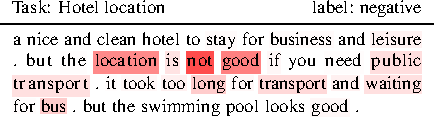
\includegraphics[width=\linewidth]{fig/attention.pdf}
\end{column}
\begin{column}{0.4\linewidth}
\vspace*{-8pt}
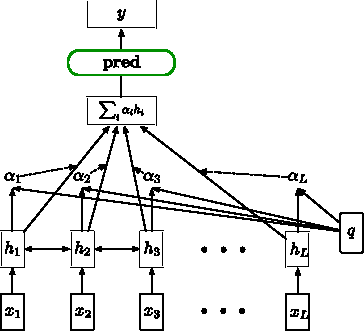
\includegraphics[width=\linewidth]{fig/attention_classifier.pdf}
\end{column}
\end{columns}
\end{frame}

\begin{frame}{Attention vs. Rationale}
\begin{lead}
    RationaleをAttention風に変換する
\end{lead}
\begin{itemize}
\item Attention $\neq$ Rationale
\begin{itemize}
    \item Attentionは連続値(強弱がある)、rationaleは二値
    \item Attentionは分類精度を最大化するよう最適化されている
\end{itemize}
\item Rationaleを直接学習に使うよりも、Rationaleを \textbf{attention 風} に変換してから学習に使うほうが良いのでは? $\Rightarrow$\emph{R2A} (rationale to attention)
\begin{itemize}
    \item 分類学習に適したAttentionを\alert{真(oracle) attention}と呼ぶ
\end{itemize}
\end{itemize}
\vspace*{-8pt}
\begin{figure}[H]
\centering
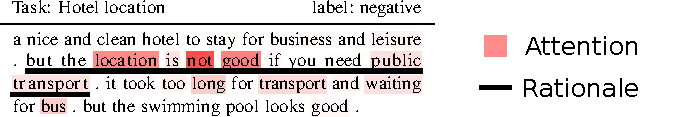
\includegraphics[width=\linewidth]{fig/attention_vs_rationale.pdf}
\end{figure}
\end{frame}

\begin{frame}{提案手法のキーポイント}
\begin{lead}
    Rationale$\Rightarrow$真attentionの変換をドメイン転移
\end{lead}
\begin{itemize}
\item 真attentionは大量の正解分類データを用い分類を学習することで獲得できる
\item 正解分類データが少ないドメイン(観点)ではRationale$\Rightarrow$真attentionの変換は学習できない
\item データが多いドメインでの変換を転移
\item 仮説:Rationale$\Rightarrow$真attentionは\alert{ドメインによらず共通}
\begin{itemize}
    \item e.g. Rationaleの中でも内容語にattentionが強くかかる
\end{itemize}
\end{itemize}
\end{frame}

\begin{frame}[c]{提案手法の流れ}
\begin{figure}[H]
  \centering
  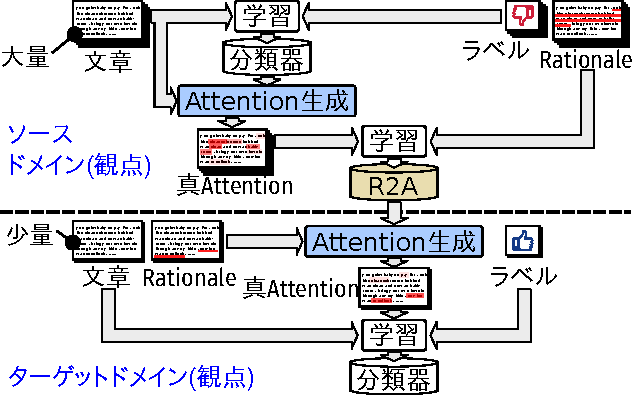
\includegraphics{fig/overview.pdf}
\end{figure}
\end{frame}

\begin{frame}[c]{問題設定(データ)}
\small
  \begin{table}
    \begin{tabular}{@{} lll @{}}
      \toprule
      データ区分 & \vtop{\hbox{\strut 分類正解}\hbox{\strut データ数}} & \vtop{\hbox{\strut rationale}\hbox{\strut 正解データ数}}\\
      \midrule
      転移元ドメイン(学習) & 大 & 大(\textbf{疑似的に生成})\\
      ターゲットドメイン(学習) & 小 & 小\\
      ターゲットドメイン(評価) & 無 & 無\\
      \bottomrule
    \end{tabular}
\end{table}
\end{frame}


\begin{frame}
\frametitle<1>{提案手法:提案手法の全体構成}
\frametitle<2>{提案手法(a)}
\frametitle<3,4>{提案手法(b)}
\frametitle<5>{提案手法(c)}
\frametitle<6>{提案手法:End-to-endな学習}
\frametitle<7>{提案手法:Attentionの転移}
\frametitle<8>{提案手法:分類器の学習}
\begin{overlayarea}{\linewidth}{60pt}
  \only<1>{
    \begin{itemize}
      \item (a) 真attentionを生成する分類器
      \item (b) 各ドメインを共通の空間にマッピング
      \item (c) attentionからrationaleを生成
    \end{itemize}
  }
  \only<2>{
    \begin{itemize}
      \item ソースドメインでattention生成と分類を学習
      \item 生成されたattentionはR2Aの正解データに
    \end{itemize}
  }
  \only<3,4>{
    \begin{itemize}
      \item 各ドメインを共通の空間にマッピング
      \begin{itemize}
        \item \texttt{enc}がリッチな特徴量を抽出できるよう言語モデル
        \item $h^{inv}$が共通の空間になるようWasserstein距離を損失に
      \end{itemize}
    \end{itemize}
  }
  \only<5>{
    \begin{itemize}
      \item Rationaleから真attentionへの変換を学習
    \end{itemize}
  }
  \only<6>{
    \begin{itemize}
      \item ソースドメインにおけるモデルをマルチタスク学習
    \end{itemize}
  }
  \only<7>{
    \begin{itemize}
      \item ソースドメインで学習したモデルを使用
      \item ターゲットドメインでRationaleから真attention を生成
    \end{itemize}
  }
  \only<8>{
    \begin{itemize}
      \item ターゲットドメインにおいて、真attentionと分類ラベルから分類器をマルチタスク学習
    \end{itemize}
  }
\end{overlayarea}


\begin{figure}
\centering
    \begin{overprint}
    \onslide<1>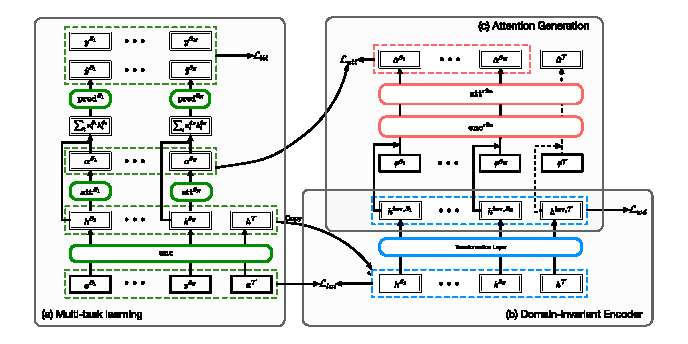
\includegraphics{fig/proposed.pdf}%
    \onslide<2>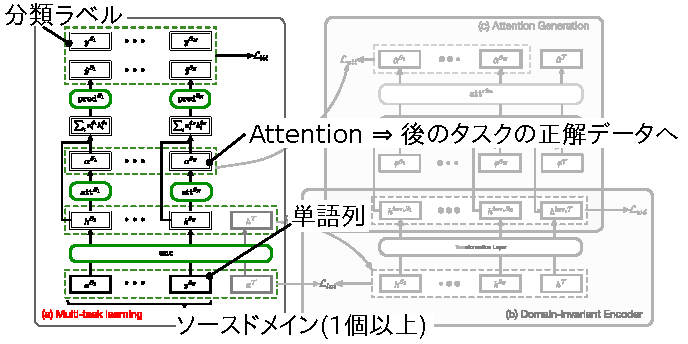
\includegraphics{fig/proposed_a.pdf}%
    \onslide<3>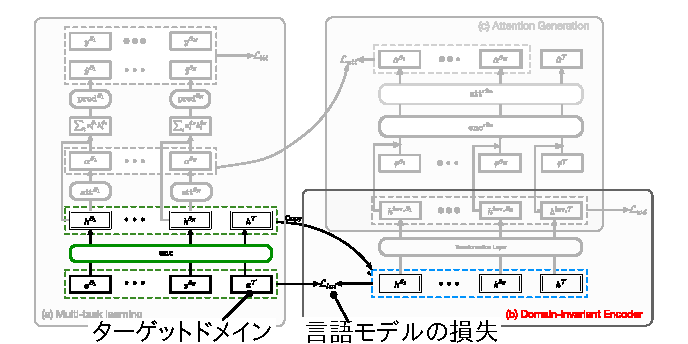
\includegraphics{fig/proposed_b1.pdf}%
    \onslide<4>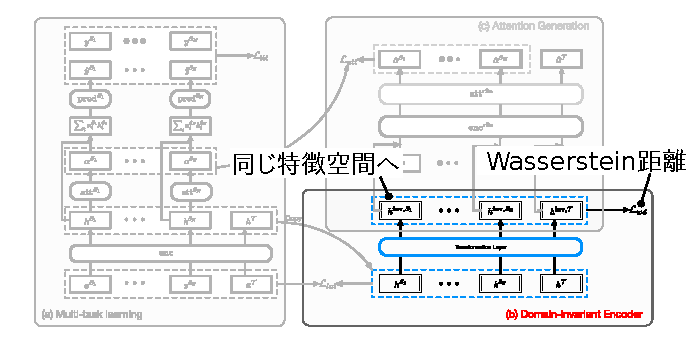
\includegraphics{fig/proposed_b2.pdf}%
    \onslide<5>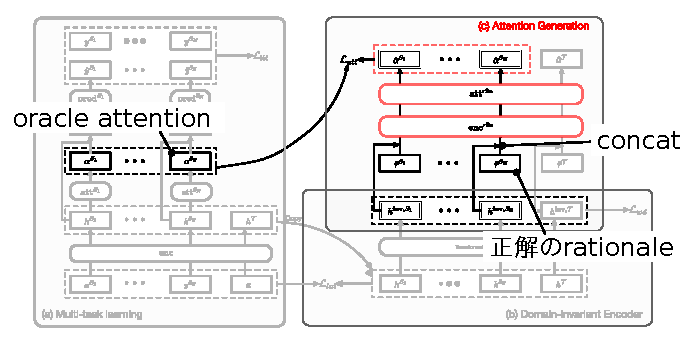
\includegraphics{fig/proposed_c.pdf}%
    \onslide<6>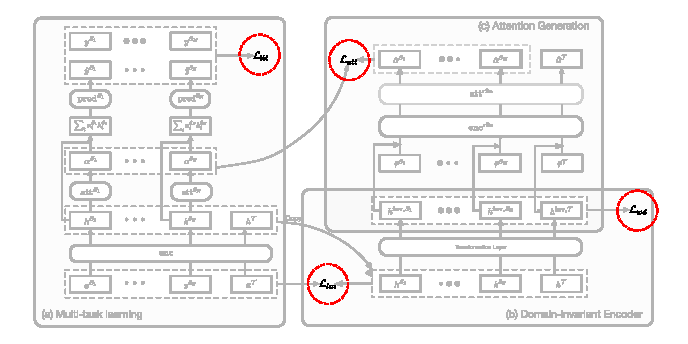
\includegraphics{fig/proposed_d.pdf}%
    \onslide<7>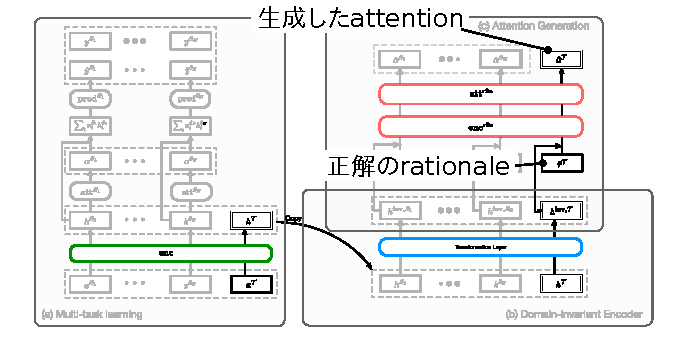
\includegraphics{fig/proposed_e.pdf}%
    \onslide<8>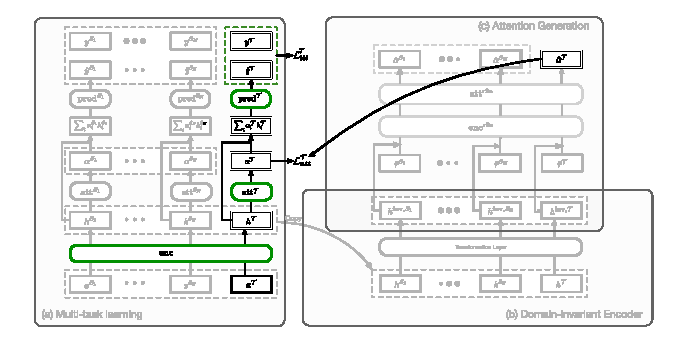
\includegraphics{fig/proposed_f.pdf}%
    \end{overprint}
\end{figure}
\end{frame}


\section{実験}
\frame[standout]{\insertsection}

\begin{frame}{観点間の転移}
\begin{lead}
    提案手法の有効性を確認
\end{lead}
\begin{itemize}
\item Rationaleを加えると分類精度が向上
\item 真attentionを介する提案手法では更に精度向上
\begin{itemize}
    \item Attention $\neq$ Rationaleを確認
\end{itemize}
\end{itemize}
\vspace*{-8pt}
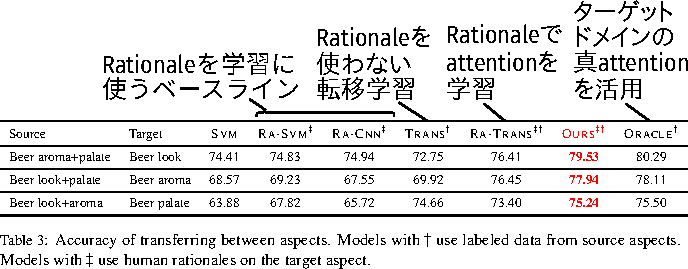
\includegraphics{fig/table3.pdf}
\end{frame}

\begin{frame}{ドメイン間の転移}
\begin{lead}
    提案手法の有効性を確認
\end{lead}
\begin{itemize}
\item ドメイン間の転移でも同様の傾向を確認
\item ターゲットドメインの真attentionを使った \textsc{Oracle}は更に性能が高い
\end{itemize}
\vspace*{-8pt}
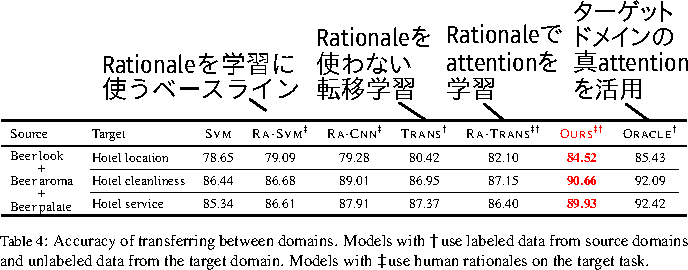
\includegraphics{fig/table4.pdf}
\end{frame}

\begin{frame}{各機能の評価}
\begin{itemize}
\item Wasserstein距離を損失を入れたモデルでは$h^{inv}$が共通の空間ある
\item Rationaleよりも、R2Aで生成したattentionのほうが真attentionに近い
\end{itemize}
\begin{columns}[onlytextwidth]
\begin{column}{0.48\linewidth}
\vspace*{-8pt}
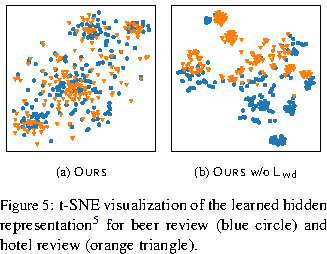
\includegraphics{fig/figure5.pdf}
\end{column}
\begin{column}{0.48\linewidth}
\vspace*{-8pt}
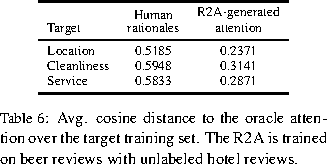
\includegraphics{fig/table6.pdf}
\end{column}
\end{columns}
\end{frame}

\begin{frame}{Rationaleを使うことの効率性}
\begin{lead}
    データを増やすよりRationaleを与える方が効率的
\end{lead}
\begin{itemize}
\item Rationaleのデータを作るくらいならばデータを増やせば良いのではないか?
\item Rationaleであれば6.5\%〜50\%のデータ量で同等の分類精度を得られる
\end{itemize}
\vspace*{-8pt}
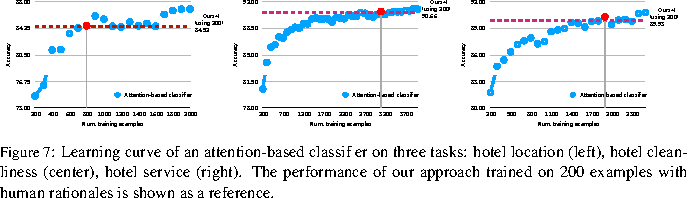
\includegraphics{fig/figure7.pdf}
\end{frame}

\section{まとめ}
\frame[standout]{\insertsection}

\begin{frame}{まとめ}
\begin{itemize}
\item Bat et al. 2018. Deriving Machine Attention from Human Rationales. EMNLP.
\item 目的:分類の根拠となった箇所のデータを用い低リソースドメインで分類精度向上
\item 手法:ドメイン非依存なRationale$\Rightarrow$attentionの変換を学習
\begin{itemize}
\item Rationale:人間が作成した分類の根拠となる記載箇所
\end{itemize}
\item 結果:観点付き評判分析の観点、ドメイン転移でベースラインを上回った
\end{itemize}
\end{frame}

\begin{frame}{コメント}

\end{frame}


\begin{frame}[c]

  Get the presentation slides from:

  \begin{center}https://bit.ly/2Us6tFn\end{center}
  \begin{center}https://github.com/koreyou/emnlp2018-meetup.git\end{center}

  This presentation is licensed under
    \href{https://creativecommons.org/publicdomain/zero/1.0/}{
    CC0 1.0 Universal (CC0 1.0) Public Domain Dedication}
    {\scriptsize (except figures derived from the original paper\cite{bao_2018})}.

  \begin{center}\cczero\end{center}

\end{frame}

\begin{frame}[allowframebreaks]{References}
  \printbibliography[heading=none]
\end{frame}

\end{document}

